\section{影响化学平衡的因素}


\begin{frame}
    \frametitle{影响化学平衡的因素}
    \begin{columns}[c]
        \column{6cm}
        \large 改变化学平衡状态
        \begin{itemize}
            \item[\bullet] 浓度$c$
            \item[\bullet] 分压$p_i$
            \item[\bullet] 总压$p$
            \item[\bullet] 加入惰性气体
        \end{itemize}
        改变平衡常数$K^\ominus$        
        \begin{itemize}
            \item[\bullet] 温度$T$
        \end{itemize}
        催化剂的影响？
        \column{6cm}
            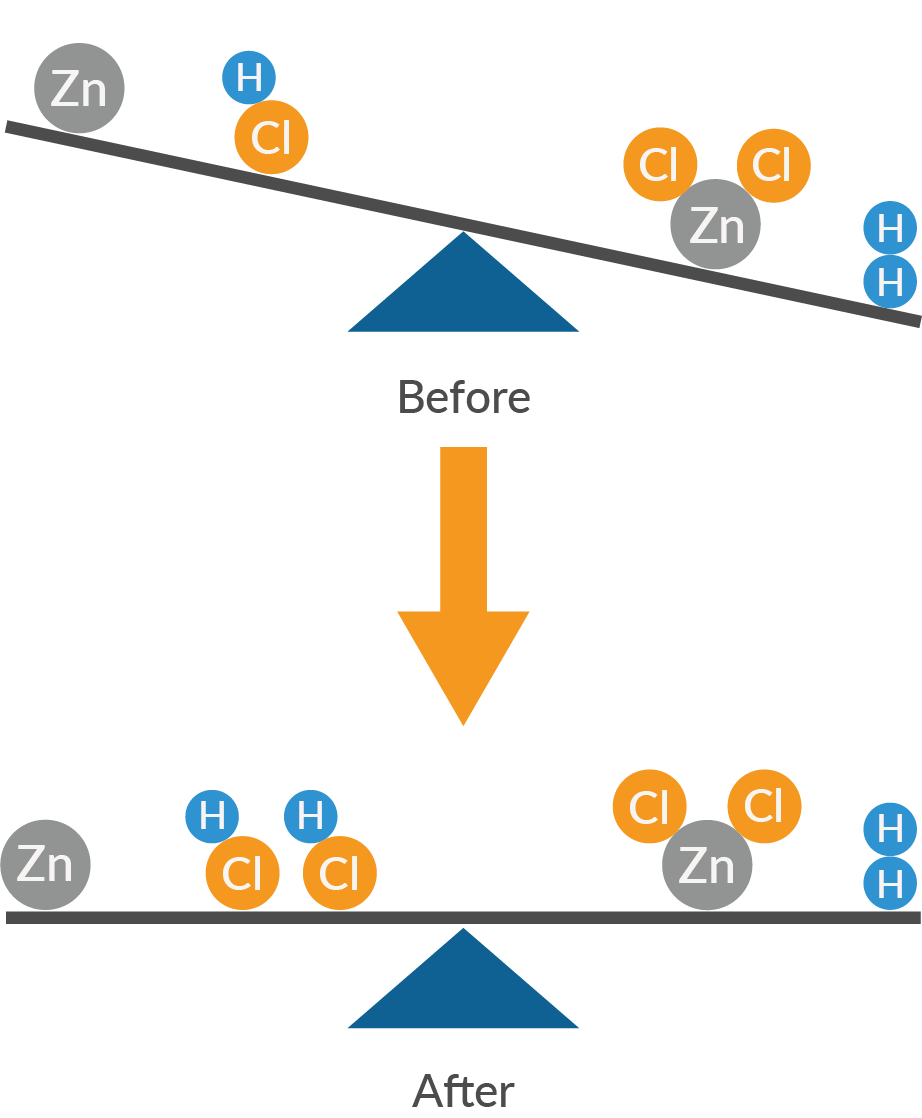
\includegraphics[height=7cm]{figs/chemical-equillibrium.png}
    \end{columns}
\end{frame}


\begin{frame}
    \frametitle{温度对$K^\ominus$的影响}

    $$\begin{aligned}
        \frac{\Delta_{\mathrm{r}} G_{\mathrm{m}}^{\ominus}}{T} &=-R \ln K^{\ominus} \qquad \qquad \text{定压下对$T$求偏微商}\\
        \frac{\partial}{\partial T}\left(\frac{\Delta_{\mathrm{r}} G_{\mathrm{m}}^{\ominus}}{T}\right)_{p} &=-R\left(\frac{\partial \ln K^{\ominus}}{\partial T}\right)_{p} \\
        \frac{\partial}{\partial T}\left(\frac{\Delta_{\mathrm{r}} G_{\mathrm{m}}^{\ominus}}{T}\right)_{p} &=-\left(\frac{\Delta_{\mathrm{r}} H_{\mathrm{m}}^{\ominus}}{T^{2}}\right)_{p} \qquad \text{吉布斯-亥姆霍兹方程，代入上式}\\
        \left(\frac{\partial \ln K^{\ominus}}{\partial T}\right)_{p} &=\frac{\Delta_{\mathrm{r}} H_{\mathrm{m}}^{\ominus}}{R T^{2}} \qquad \qquad \quad \text{因标准平衡常数只是温度的函数}\\
        \frac{\mathrm{d} \ln K^{\ominus}}{\mathrm{d} T} &=\frac{\Delta_{\mathrm{r}} H_{\mathrm{m}}^{\ominus}}{R T^{2}} \qquad \qquad \quad \text{范特霍夫方程}
    \end{aligned}$$

\end{frame}


\begin{frame}
    \frametitle{温度对$K^\ominus$的影响}
    \[
        \frac{\mathrm{d} \ln K^{\ominus}}{\mathrm{d} T} =\frac{\Delta_{\mathrm{r}} H_{\mathrm{m}}^{\ominus}}{R T^{2}}
    \]
    \begin{itemize}
        \item[(1)] 对吸热反应，$\Delta_{\mathrm{r}} H_{\mathrm{m}}>0$，$\mathrm{d} \ln K^{\ominus}/{\mathrm{d} T}>0$
        \begin{itemize}
            \item[\bullet] 当温度升高时，标准平衡常数$K^\ominus$变大，平衡向增加产物方向移动；
            \item[\bullet] 当温度降低时，$K^\ominus$变小，平衡向增加反应物方向移动。
        \end{itemize}
        \item[(2)] 对放热反应，$\Delta_{\mathrm{r}} H_{\mathrm{m}}<0$，$\mathrm{d} \ln K^{\ominus}/{\mathrm{d} T}<0$
        \begin{itemize}
            \item[\bullet] 当温度升高时，$K^\ominus$变小，平衡向增加反应物方向移动；
            \item[\bullet] 当温度降低时，$K^\ominus$变大，平衡向增加产物方向移动。
        \end{itemize}       
    \end{itemize}

\end{frame}


\begin{frame}
    \frametitle{温度对$K^\ominus$的影响}

    温度变化不大时，视$\Delta_{\mathrm{r}} H_{\mathrm{m}}^\ominus$为常数
    
    范特霍夫方程不定积分式：
    \[
        \ln K^{\ominus}=-\frac{\Delta_{\mathrm{r}} H_{\mathrm{m}}^{\ominus}}{R T}+c
    \]
    测得某反应一系列温度下的$K^\ominus$值，以$\ln K^\ominus$对$1/T$作图得一直线，由直线斜率可求反应$\Delta_{\mathrm{r}} H_{\mathrm{m}}$。

    范特霍夫方程定积分式：
    \[
        \ln \frac{K_{2}^{\ominus}}{K_{1}^{\ominus}}=\frac{\Delta_{\mathrm{r}} H_{\mathrm{m}}^{\ominus}}{R}\left(\frac{1}{T_{1}}-\frac{1}{T_{2}}\right)
    \]
    根据反应$T_1$时的$K_1^\ominus$及$\Delta_{\mathrm{r}} H_{\mathrm{m}}^\ominus$可求$T_2$时的$K_2^\ominus$。

\end{frame}


\begin{frame}
    \frametitle{为什么范特霍夫方程和克-克方程形式如此相似？}

    \large 范特霍夫方程
    \[
        \frac{\mathrm{d} \ln K^{\ominus}}{\mathrm{d} T} =\frac{\Delta_{\mathrm{r}} H_{\mathrm{m}}^{\ominus}}{R T^{2}}
    \]
    克劳修斯-克拉贝龙方程
    \[
        \frac{\mathrm{d} \ln p}{\mathrm{~d} T}=\frac{\Delta H_\mathrm{m}}{RT^2}
    \]
    两者的推导同源，都是源于热力学基本方程$\mathrm{d}G=-S\mathrm{d}T+V\mathrm{d}p$，只不过前者是在化学平衡条件下推导（结合等温方程），后者则是在相平衡下推导（两相化学势相等），所以两者形式上相似。

\end{frame}


\begin{frame}[t]
    \frametitle{}

    \begin{example}
        已知\ch{CaCO3}在\SI{1170}{K}时的分解压力为\SI{100.0}{kPa}，反应\ch{CaCO3(s) = CaO(s) + CO2(g)}的$\Delta_{\mathrm{r}} H_{\mathrm{m}}$在本题计算范围内恒定为\SI{170.8}{kJ.mol^{-1}}。若空气中\ch{CO2}的摩尔分数为0.3\%，计算\ch{CaCO3}在空气中开始分解的温度。
    \end{example}
    \pause
    $$\begin{array}{c}
        K^{\ominus}=p_{\mathrm{CO}_{2}} / p^{\ominus} \\
        K_{1}^{\ominus}=100.0 \mathrm{kPa} / 100.0 \mathrm{kPa}=1 \\
        K_{2}^{\ominus}=0.003 p^{\ominus} / p^{\ominus}=0.003 \\
        \ln \frac{K_{2}^{\ominus}}{K_{1}^{\ominus}}=\frac{\Delta_{\mathrm{r}} H_{\mathrm{m}}^{\ominus}}{R}\left(\frac{1}{T_{1}}-\frac{1}{T_{2}}\right) \\
        \ln \frac{0.003}{1}=\frac{1.708 \times 10^{5} \mathrm{~J} \cdot \mathrm{mol}^{-1}}{8.314 \mathrm{~J} \cdot \mathrm{mol}^{-1} \cdot \mathrm{K}^{-1}}\left(\frac{1}{1170 \mathrm{~K}}-\frac{1}{T_{2}}\right) \\
        T_{2}=879 \mathrm{~K}
        \end{array}$$

\end{frame}


\begin{frame}[t]
    \frametitle{}

    \begin{example}
        反应\ch{C(s) + H2O(g) <=> H2(g) + CO(g)}若在1000K及1200K时的$K^{\ominus}$分别为2.472及37.58。试计算在此温度范围内的平均反应热$\Delta_{\mathrm{r}} H_{\mathrm{m}}^\ominus$及在1100K时的标准平衡常数$K^{\ominus}$。
    \end{example}
    \pause
    \[
        \ln \frac{K^{\ominus}(1200 K)}{K^{\ominus}(1000 K)}=\frac{\Delta_{\mathrm{r}} H_{\mathrm{m}}^\ominus}{R}\left(\frac{1}{1000}-\frac{1}{1200}\right)
    \]
    \[
        \Delta_{\mathrm{r}} H_{\mathrm{m}}^\ominus=135.76 \mathrm{~kJ} \cdot \mathrm{mol}^{-1}
    \]
    \[
        \ln \frac{K^{\ominus}(1100 K)}{2.472}=\frac{135760}{8.314}\left(\frac{1}{1000}-\frac{1}{1100}\right)
    \]
    \[
        K^{\ominus}(1100 K)=10.91
    \]

\end{frame}